\documentclass{article}
\usepackage{amssymb}
\usepackage{amsmath}
\usepackage{mathtools}
\usepackage{cancel}
\usepackage{tikz}
\usepackage{hyperref}
\usepackage{circuitikz}
\usepackage{float}
\usepackage{afterpage}
\usepackage{pgfplots}
\usetikzlibrary{calc, arrows}
\newtheorem{theorem}{Theorem}
\newtheorem{definition}{Definition}
\newtheorem{corollary}{Corollary}
\newtheorem{proof}{Proof}
\tikzstyle{int}=[draw, fill=blue!20, minimum size=2em]
\tikzstyle{init} = [pin edge={to-,thin,black}]

\DeclareMathOperator*{\argmin}{argmin}

\begin{document}
\title{EE120 Course Notes}
\author{Anmol Parande}
\date{Fall 2019 - Professor Murat Arcak}
\maketitle
\textbf{Disclaimer: }These notes reflect 120 when I took the course (Fall 2019). They may not accurately reflect current course content, so use at your own risk.
If you find any typos, errors, etc, please raise an issue on the \href{https://github.com/parandea17/BerkeleyNotes}{GitHub repository}.\\
\tableofcontents
\newpage
\section{Introduction to Signals and Systems}
\subsection{Types of Signals}
\begin{definition}
    A signal is a function of one or more variables
\end{definition}
\begin{definition}
    A continuous signal $x(t)$ maps $\mathbb{R} \rightarrow \mathbb{R}$
\end{definition}
\begin{definition}
    A discrete signal $x[n]$ maps $\mathbb{Z} \rightarrow \mathbb{R}$
\end{definition}
\subsubsection{Properties of the Unit Impulse}
\begin{definition}
    The unit impulse in discrete time is defined as 
    \[
        \delta[n] = \left\{
            \begin{array}{cc}
                1, \text{if } n=0\\
                0, \text{ else}
            \end{array}
            \right\}
    \]
\end{definition}
\begin{itemize}
    \item $f[n]\delta[n] = f[0]\delta[n]$
    \item $f[t]\delta[n-N] = f[N]\delta[n-N]$
\end{itemize}
\begin{definition}
    The unit impulse in continuous time is the dirac delta function
    $$\delta(t)=lim_{\Delta\rightarrow 0}\delta_{\Delta}(t)$$
    \[
        \delta_{\Delta}=\left\{
            \begin{array}{c}
                \frac{1}{\Delta},\text{ if }\ge 0 \\
                0 else
            \end{array}
        \right\}
    \]
\end{definition}
\begin{itemize}
    \item $f(t)\delta(t) = f(0)\delta(t)$
    \item $f(t)\delta(t-\tau) = f(\tau)\delta(t-\tau)$
    \item $\delta(at) = \frac{1}{|a|}\delta(t)$
\end{itemize}
\begin{definition}
    The unit step is defined as 
    \[
        u[n] = \left\{
            \begin{array}{cc}
                1, \text{if } n \geq 0\\
                0, \text{ else}
            \end{array}
            \right\}
    \]
\end{definition}
\subsection{Signal transformations}
Signals can be transformed by modifying the variable.
\begin{itemize}
    \item $x(t - \tau)$: Shift a signal left by $\tau$ steps.
    \item $x(-t)$: Rotate a signal about the $t=0$
    \item $x(kt)$: Stretch a signal by a factor of $k$
\end{itemize}
These operations can be combined to give more complex transformations.
For example, $y(t) = x(\tau - t) = x(-(t-\tau))$ flips $x$ and shifts it right by $\tau$ timesteps.
This is equivalent to shifting $x$ left by $\tau$ timesteps and then flipping it.
\subsection{Convolution}
\begin{definition}
    The convolution of two signals in discrete time
    $$(x*h)[n] = \sum_{k=-\infty}^{\infty}{x[k]h[n-k]}$$
\end{definition}
\begin{definition}
    The convolution of two signals in continuous time
    $$(x*h)(t) = \int_{-\infty}^{\infty}{x(\tau)h(t-\tau)d\tau}$$
\end{definition}
While written in discrete time, these properties apply in continuous time as well.
\begin{itemize}
    \item $(x*\delta)[n] = x[n]$
    \item $x[n]*\delta[n-N]=x[n-N]$
    \item $(x*h)[n] = (h*x)[n]$
    \item $x * (h_1 + h_2) = x*h_1 + x*h_2$
    \item $x * (h_1 * h_2) = (x * h_1) * h_2$
\end{itemize}
\subsection{Systems and their properties}
\begin{definition}
    A system is a process by which input signals are transformed to output signals
\end{definition}
\begin{definition}
    A memoryless system has output which is only determined by the input's present value
\end{definition}
\begin{definition}
    A causal system has output which only depends on input at present or past times
\end{definition}
\begin{definition}
    A stable system produces bounded output when given a bounded input. By extension,
    this means an unstable system is when $\exists$ a bounded input that makes the output unbounded.
\end{definition}
\begin{definition}
    A system is time-invariant if the original input $x(t)$ is transformed to $y(t)$, then
    $x(t-\tau)$ is transformed to $y(t-\tau)$
\end{definition}
\begin{definition}
    A system $f(x)$ is linear if and only if
    \begin{itemize}
        \item If $y(t) = f(x(t))$, then $f(a x(t)) = a y(t)$ (Scaling)
        \item If $y_1(t) = f(x_1(t))$ and $y_2(t) = f(x_2(t))$, then $f(x_1(t) + x_2(t)) = y_1(t) + y_2(t)$ (Superposition)
    \end{itemize}
\end{definition}
\textbf{Notice: } The above conditions on linearity require that $x(0) = 0$ because if $a = 0$, then we need $y(0) = 0$ for scaling to be satisfied
\begin{definition}
    The impulse response of a system $f[x]$ is $h[n] = f[\delta[n]]$, which is how it response to an impulse input. 
\end{definition}
\begin{definition}
    A system has a Finite Impulse Response (FIR) if $h[n]$ decays to zero in a finite
    amount of time
\end{definition}
\begin{definition}
    A system has an Infinite Impulse Response (IIR) if $h[n]$ does not decay to zero in a finite
    amount of time
\end{definition}
\subsection{Exponential Signals}
Exponential signals are important because they can succinctly represent
complicated signals using complex numbers. This makes analyzing them much easier.
$$x(t) = e^{st}, x[n] = z^n (s, z \in \mathbb{C})$$
\begin{definition}
    The frequency response of a system is how a system responds to a purely oscillatory signal
\end{definition}
\section{The Fourier Series}
\subsection{Continuous Time}
\begin{definition}
    A function $x(t)$ is periodic if $\exists T$ such that $\forall t, x(t-T)=x(t)$.
\end{definition}
The smalled such $T$ which satisfies the periodicity property is known as the \textbf{Fundamental Period}.
\begin{theorem}
    If $x(t)$ and $y(t)$ are functions with period $T_1$ and $T_2$ respectively, then $x(t)+y(t)$ is periodic
    if $\exists m, n \in \mathbb{Z}$ such that $mT_1 = nT_2$.
\end{theorem}
\begin{definition}
    Given a periodic function $x(t)$ with fundamental period $T$ and fundamental frequency $\omega_0=\frac{2\pi}{T}$,
    the Fourier Series of $x$ is a weighted sum of the harmonic functions.
    $$x(t) = \sum_{k=-\infty}^{\infty}{a_ke^{jk\omega_0t}}$$
\end{definition}
To find the coefficients $a_k$:
$$x(t) \cdot e^{-jn\omega_0t} = \sum_{k=-\infty}^{\infty}{a_ke^{j\omega_0t(k-n)}}$$
\[
    \int_{T}{x(t) \cdot e^{-jn\omega_0t}dt} = \sum_{k=-\infty}^{\infty}{a_k\int_{T}{e^{j\omega_0t(k-n)}}dt}
    = \left\{
        \begin{array}{cc}
            Ta_k & \text{if }$k=n$\\
            0 & \text{else}
        \end{array}
    \right\}
\]
Rearranging this, we can see that
$$a_n = \frac{1}{T}\int_{T}{x(t)e^{-jn\omega_0t}dt}$$.
For $a_0$, the DC offset term, this formula makes a lot of sense because it is just the average value of the function over one period.
$$a_0 = \frac{1}{T}\int_{T}{x(t)dt}$$
Because the Fourier Series is an infinite sum, there is a worry that for some functions $x(t)$, it will not converge.
The \textbf{Dirichlet Convergent Requirements} tell us when the Fourier Series converges.
More specificially, they tell us when
$$\lim_{M \rightarrow \infty}{x_M(\tau) = x(\tau)} \forall \tau, x_M(t) = \sum_{k=-M}^{M}{a_k e^{jk\omega_0t}}$$
will converge.
\begin{theorem}
    The Fourier Series of a continuous time periodic function $x(t)$ will converge when
    $x$ is piecewise continuous and $\frac{d}{dt}x$ is piecewise continuous.
    \begin{itemize}
        \item If $x$ is continuous at $\tau$, $\lim_{M \rightarrow \infty}x_M(\tau) = x(\tau)$
        \item If $x$ is discontinuous at $\tau$, then $\lim_{M\rightarrow \infty}x_M(\tau) = \frac{1}{2}(x(\tau^- + x(\tau^+)))$ 
    \end{itemize}
\end{theorem}
These convergence requirements are for pointwise convergence only. They do not necessarily imply that the graphs of the Fourier Series
and the original function will look the same.
\subsection{Discrete Time}
The definition for periodicity in discrete time is the exact same as the definition in continuous time.
\begin{definition}
    A function $x[n]$ is periodic with period $N \in \mathbb{Z}$ if $\forall n, x[n+N]=x[n]$
\end{definition}
However, there are some differences. For example, $x[n] = cos(\omega_0 n)$
is only periodic in discrete time if $\exists N, M \in \mathbb{Z}, \omega_0 N = 2 \pi M$.
\begin{theorem}
    The sum of two discrete periodic signals is periodic
\end{theorem}
The above statement is not always true in continuous time but it is in discrete time.\\\\
The Fourier Series in discrete time is the same idea as the Fourier series in continuous time: 
to express every signal as a linear combination of complex exponentials.
The discrete time basis that we use are the Nth roots of unity.
$$\phi_k[n] = e^{jk\frac{2\pi}{N}n}$$
\begin{itemize}
    \item $\phi_k[n]$ is perioidic in n (i.e $\phi_k[n+N] = \phi_k[n]$)
    \item $\phi_k[n]$ is periodic in k (i.e $\phi_{k+N}[n] = \phi_k[n]$)
    \item $\phi_k[n]\cdot \phi_m[n] = \phi_{k + m}[n]$
\end{itemize}
Notice that with this basis, there are only N unique functions that we can use.
An additional property of the $\phi_k[n]$ is that
\[
    \sum_{n=<N>}{\phi_k[n]} = \left\{
        \begin{array}{cc}
            N &\text{if } k = 0,\pm N, \pm 2N\\
            0 &\text{otherwise} 
        \end{array}
    \right\}
\]
\begin{definition}
    Given a periodic discrete-time function $x[n]$ with period $N$, 
    the Fourier series of the function is a weighted sum of the roots of unity basis functions.
    $$x[n] = \sum_{k=0}^{N-1}{a_k\phi_k[n]}$$
\end{definition}
In order to find the values of $a_k$, we can perform a similar process as in continuous time.
$$x[n] = \sum_{k=0}^{N-1}{a_k\phi_k[n]}$$
$$x[n]\phi_{-M}[n] = \sum_{k=0}^{N-1}{a_k\phi_k[n]\phi_{-M}[n]}$$
$$\sum_{n=<N>}{x[n]\phi_{-M}[n]} = \sum_{n=<N>}{\sum_{k=<N>}{a_k\phi_{k-M}[n]}} = \sum_{k=<N>}{a_k\sum_{n=<N>}{\phi_{k-M}[n]}}$$
$$\sum_{n=<N>}{x[n]\phi_{-M}[n]} = a_MN$$
$$a_M = \frac{1}{N}\sum_{n=<N>}{x[n]\phi_{-M}[n]}$$
\subsection{Properties of the Fourier Series}
\textbf{Linearity: }
If $a_k$ and $b_k$ are the coefficients of the Fourier Series of $x(t)$ and $y(t)$ respectively, then
$Aa_k + Bb_k$ are the coefficients of the Fourier series of $Ax(t)+By(t)$\\\\
\textbf{Time Shift: }
If $a_k$ are the coefficients of the Fourier Series of $x(t)$,
then $b_k = e^{-jk\frac{2\pi}{T}t_0}a_k$ are the coefficients of the Fourier Series of $\hat{x}(t)=x(t-t_0)$\\\\
\textbf{Time Reversal: }
If $a_k$ are the coefficients of the Fourier Series of $x(t)$,
then $b_k=a_{-k}$ are the coefficients of the Fourier Series of $x(-t)$\\\\
\textbf{Conjugate Symmetry: }
If $a_k$ are the coefficients of the Fourier Series of $x(t)$,
then $a_k^*$ are the coefficients of the Fourier Series of $x^*(t)$. 
This means that $x(t)$ is a real valued signal, then $a_k=a_{-k}^*$
\begin{theorem}[Parseval's Theorem]
    \begin{equation*}
        \frac{1}{T}\int{|x(t)|^2dt} = \sum_{k=-\infty}^{\infty}{|a_k|^2} (Continous Time)
    \end{equation*}
    \begin{equation*}
        \frac{1}{N}\sum_{n=<N>}{|x[n]|^2} = \sum_{k=<N>}{|a_k|^2} (Discrete Time)
    \end{equation*}
\end{theorem}
\subsection{Interpreting the Fourier Series}
A good way to interpret the Fourier Series is as a change of basis. In both the continuous and discrete case,
we are projecting our signal $x$ onto a set of basis functions, and the coefficients $a_k$ are the coordinates
of our signal in the new space.
\subsubsection{Discrete Time}
Since in discrete time, signal is peroidic in $N$, we can turn any it into a vector $\vec{x}\in \mathbb{C}^N$.
\[
    \vec{x} = \left[
        \begin{array}{c}
            x[0]\\
            x[1]\\
            \vdots\\
            x[N-1]
        \end{array}
    \right] \in \mathbb{C}^N
\]
We can use this to show that $\phi_k$ form an orthogonal basis.
If we take two of them $\phi_k[n]$ and $\phi_M[n]$ ($k\ne M$) and compute their dot product of their vector forms, then
$$\phi_k[n] \cdot \phi_M[n] = \phi_M^*\phi_k = \sum_{<n>}{\phi_{k-M}[n]} = 0$$
That means that $\phi_k$ and $\phi_M$ are orthogonal, and they are $N$ of them, therefore they are a basis.
If we compute their magnitudes, we see
$$\phi_k \cdot \phi_k = ||\phi_k||^2 = N, \therefore ||\phi_k|| = \sqrt{N}$$
Finally, if we compute $\vec{x}\phi_M$ where $\vec{x}$ is the vector form of an N-periodic signal,
$$\vec{x}\cdot \vec{\phi_M} = (\sum_{i=0}^{N-1}{a_i\phi_i})\cdot \phi_M = Na_m$$
$$a_m = \frac{1}{N}\vec{x}\cdot \phi_M$$
This is exactly the equation we use for finding the Fourier Series coefficients, and notice that it is a
projection since $N = ||\phi_m||^2$. This gives a nice geometric intution for Parseval's theorem.
$$\frac{1}{N}\sum{|x[n]|^2} = \frac{1}{N}||\vec{x}||^2 = \sum{|a_k|^2}$$
because we know the norms of two vectors in different bases must be equal.
\subsubsection{Continuous Time}
In continuous time, our bases functions are $\phi_k(t) = e^{jk\frac{2\pi}{T}t}$ for $k \in (-\infty, \infty)$
Since we can't convert continuous functions into vectors, these $\phi_k$ are really a basis for the vector space
of square integrable functions on the interval $[0, T]$.
The inner product for this vector space is 
$$<x, y> = \int_{0}^{T}{x(t)y^*(t)}$$
We can use this inner product to conduct the same proof as we did in discrete time.
\section{The Fourier Transform}
\subsection{Continuous Time Fourier Transform}
\begin{definition}
    The Continuous Time Fourier Transform converts an aperiodic signal into the frequency domain.
    $$X(\omega) = \int_{-\infty}^{\infty}{x(t)e^{-j\omega t}dt}$$
\end{definition}
The intuition for this transform comes from the Fourier Series. Only periodic signals can be represented by the Fourier Series.
If we start with a finite signal $x(t)$, then we can just make it periodic by copying the domain over which it is nonzero so 
it repeats over a period $T$. Call this signal $\tilde{x}(t)$. Since $\tilde{x}$ is perioidc,
we can find its fourier series coefficients.
\[
    a_k = \frac{1}{T}\int_{T}{\tilde{x}(t)e^{-jn\frac{2\pi}{T}t}} = 
    \frac{1}{T}\int_{T}{x(t)e^{-jn\frac{2\pi}{T}t}} = \frac{1}{T}\int_{-\infty}^{\infty}{x(t)e^{-jn\frac{2\pi}{T}t}}
\]
These steps are possible because $\tilde{x}(t) = x(t)$ over a single period, and $x(t)$ is zero outside that period.
$$Ta_k = \int_{-\infty}^{\infty}{x(t)e^{-jn\frac{2\pi}{T}t}}$$
notice that if we let $T$ approach infinity, then $\omega_0 = \frac{2\pi}{T}$ becomes very small, so the $Ta_k$
can almost be thought of as samples of some continuous time function. What this means is for a general aperiodic signal,
regardless of if it is finite or not, we can think of it as having "infinite period" and thus made up of a continuous set of frequencies.
This is what motivates the continuous time fourier transform.
\begin{definition}
    The Inverse Continuous Time Fourier Transform takes us from the frequency domain
    reprsentation of a function $X(\omega)$ to its time domain representation $x(t)$
    $$x(t) = \frac{1}{2\pi}\int_{-\infty}^{\infty}{X(\omega)e^{j\omega t}d\omega}$$
\end{definition}
We can arrive at this equation by starting from the Fourier series again
Our faux signal $\tilde{x}(t)$ which was the periodic function we constructed out of our aperiod one
is represented by its Fourier Series
$$\tilde{x}(t) = \sum_{k-\infty}^{\infty}{a_ke^{jk\omega_0t}} = \sum_{k=-\infty}^{\infty}{(\frac{1}{T}X(\omega))e^{j\omega t}}|_{w=k\omega_0}$$
Notice this is just rewrite $a_k$ as the samples of the Fourier Transform $X(\omega)$. $T = \frac{2\pi}{\omega_0}$ so
$$\tilde{x}(t) = \frac{1}{2\pi} \sum_{k=-\infty}^{\infty}{\omega_0X(\omega)e^{j\omega t}}|_{w=k\omega_0}$$
$$x(t) = \lim_{T->\infty}{\tilde{x}(t)} = lim_{\omega_0->0}{\tilde{x}(t)} = \frac{1}{2\pi}\int_{-\infty}^{\infty}{X(\omega)e^{j\omega t}d\omega}$$
\subsubsection{Properties of the CTFT}
For all these properties, assume that $x(t) \leftrightarrow X(\omega)$ and $y(t) \leftrightarrow Y(\omega)$\\
\textbf{Linearity: } 
$$ax(t) + by(t) \leftrightarrow aX(\omega) + bY(\omega)$$
\textbf{Time Shift: }
$$x(t-t_0) \leftrightarrow e^{-j\omega t_0}X(\omega)$$
\textbf{Time/Frequency Scaling: }
$$x(at) \leftrightarrow \frac{1}{|a|}X(\frac{\omega}{a})$$
\textbf{Conjugation: } 
$$x^*(t) \leftrightarrow X^*(-\omega)$$
\textbf{Derivative: } 
$$\frac{d}{dt}x(t) \leftrightarrow j\omega X(\omega), \frac{d}{d\omega}X(\omega) \leftrightarrow -jt x(t)$$
\textbf{Convolution/Multiplication: } 
$$(x*y)(t) \leftrightarrow X(\omega)Y(\omega), x(t)y(t) \leftrightarrow \frac{1}{2\pi}(X*Y)(\omega)$$
\textbf{Frequency Shift: } 
$$e^{j\omega_0 t}x(t) \leftrightarrow X(\omega - \omega_0)$$
\textbf{Parsevals Theorem: }
$$\int_{-\infty}^{\infty}{|x(t)|^2dt} = \frac{1}{2\pi}\int_{-\infty}^{\infty}{|X(\omega)|^2d\omega}$$
\subsubsection{Convergence of the CTFT}
A big question that arises when thinking about the Fourier Transform is whether or not the integral $\int{x(t)e^{-j\omega t}}$
actually converges.
\begin{theorem}
    If $\int_{-\infty}^{\infty}{|x(t)|dt}$ converges, then $X(\omega)$ exists and is continuous.
    In addition, $X(\omega)$ approaches 0 as $|\omega|$ approaches $\infty$
\end{theorem}
Conceptually, this theorem makes sense because
$$|x(t)e{-j\omega t}| = |x(t)| |e^{-j\omega t}| = |x(t)|$$
So if one converges, the other must converge. However, this means that $x(t)=1$, $x(t)=sin(\omega t)$, $x(t)=cos(\omega t)$
don't have a "strict" Fourier Series because the integral doesn't converge for these periodic signals. In order to get around this,
we can define a "generalized" Fourier Transform which operates on periodic signals.\\\\
Starting with $x(t)=1$, we know that in the frequency domain, the only consituent frequency is $\omega=0$.
This means that $X(\omega) = k\delta(\omega)$ where $k$ is some scalar.
Using the Inverse Fourier Transform,
$$x(t) = \frac{1}{2\pi}\int{k\delta(\omega)e^{j\omega t}d\omega} = \frac{k}{2\pi}$$
That means $k = 2\pi$, so
$$x(t) = 1 \leftrightarrow X(\omega) = 2\pi \delta(\omega)$$
Now if we apply the frequency shift property, we see that
$$x(t) = e^{j\omega_0 t} = 2\pi \delta(\omega - \omega_0)$$
With this, we can define our generalized Fourier Transform for periodic signals.
\begin{definition}
    The generalized Fourier Transform for a periodic signal $x(t)$ is
    $$X(\omega) = \sum_{-\infty}^{\infty}{a_k\cdot 2\pi \delta(\omega - \omega_0)}$$
    where $a_k$ are the coefficients of the Fourier Series of $x(t)$
\end{definition}
This definition works because any periodic signal can be represented by its Fourier Series.
The rational behind using the Dirac Delta in this generalized Fourier Transform is exlained by the 
Theory of Distributions which can be found in the Appendix. %TODO: Link to Appendix
\subsection{Discrete Time Fourier Transform}
\begin{definition}
    The Discrete Time Fourier Transform converts aperiodic discrete signals into the frequency domain.
    $$X(\omega) = \sum_{-\infty}^{\infty}{x[n]e^{-j\omega n}}$$
\end{definition}
The intution for the discrete time fourier transform is more or less the same as that of the Continuous Time Fourier Transform.
\begin{definition}
    The Inverse Discrete Time Fourier Transform converts the frequency domain representation of a signal
    back into its time domain representation.
    $$x[n] = \frac{1}{2\pi}\int_{<2\pi>}{X(\omega)e^{j\omega n}d\omega}$$
\end{definition}
\subsubsection{Properties of the DTFT}
For all these properties, assume that $x[n] \leftrightarrow X(\omega)$ and $y[n]\leftrightarrow (\omega)$\\
\textbf{Time Shift: }
$$ x[n-n_0] \leftrightarrow e^{-j\omega n_0}X(\omega)$$
\textbf{Frequency Shift: }
$$ X(\omega - \omega_0) \leftrightarrow e^{j\omega_0 n}x[n]$$
\textbf{Time Reversal: }
$$ x[-n] \leftrightarrow X(-\omega)$$
\textbf{Conjugation: }
$$ x^*[n] = X^*(-\omega)$$
\textbf{Time Expansion: }\\
In discrete time, compression of a signal doesn't make sense because we can't have partial steps (i.e n must be an integer).
However, we can stretch a signal.
\[
    x_M[n] \leftrightarrow X(M\omega), x_M[n] = \left\{
        \begin{array}{cc}
            x[\frac{n}{M}] & \text{when } M | n\\
            0 & \text{else}
        \end{array}
    \right\}
\]
\textbf{Derivative Property: }
$$nx[n] \leftrightarrow j \frac{d}{d\omega}X(\omega)$$
\textbf{Multiplication Property: }
$$ x[n]y[n] \leftrightarrow \frac{1}{2\pi}\int_{2\pi}{X(\theta)Y(\omega-\theta)d\theta}$$
\textbf{Convolution Property: }
$$(x*y)[n] = X(\omega)Y(\omega)$$
\subsubsection{Convergence of the DTFT}
Just like in continuous time, it was unclear whether or not the integral would converge,
in discrete time, it is unclear if the infinite sum will converge. The convergence theorem for both are essentially the same.
\begin{theorem}
    If $\sum_{-\infty}^{\infty}{|x[n]|}$ converges, then $X(\omega)$ exists and is continuous.
\end{theorem}
Just like in continuous time, periodic signals like $x[n] = 1, x[n] = sin(\omega_0t), x[n]=cos(\omega_0t)...$
are problematic because they don't converge under the "strict" transform, so they require a generalied transform.
In the frequency domain, a constant signal like $x[n] = 1$ will be the sum of all frequencies. This will look like
a sum of Dirac Deltas.
$$X(\omega) = k \sum_{l=-\infty}^{\infty}{\delta(\omega - 2\pi l)}$$
Applying the synthesis equation to this, we get
$$x(t) = \frac{1}{2\pi}\int_{2\pi}{k \sum_{l=-\infty}^{\infty}{\delta(\omega - 2\pi l)}} = \frac{k}{2\pi}\sum_{l=-\infty}^{\infty}{\int_{2\pi}{\delta(\omega - 2\pi l)}} = \frac{k}{2\pi}\int_{2\pi}{\delta(\omega - 2\pi \cdot 0)} = \frac{k}{2\pi}$$
Therefore $k = 2\pi$, so
$$x[n] = 1 \leftrightarrow X(\omega) = 2\pi\sum_{l=-\infty}^{\infty}{\delta(\omega - 2\pi l)}$$
and we can apply the frequency shift property to get
$$x[n] = e^{j\omega_0n} \leftrightarrow X(\omega) = 2\pi\sum_{l=-\infty}^{\infty}{\delta(\omega - \omega_0 - 2\pi l)}$$
Once again using the Fourier Series representation of $x[n]$, we can define the generalized Discrete Time Fourier Transform.
\begin{definition}
    For a perioidic signal $x[n]$, the generalized Discrete Time Fourier Transform is
    $$x[n] \leftrightarrow 2\pi\sum_{-\infty}^{\infty}{a_k\delta(\omega-\frac{2\pi}{N}k)}$$
    where $a_k$ are the Fourier Series coefficients of $x[n]$
\end{definition}
\subsection{Discrete Fourier Transform}
Whereas the CTFT takes a continuous signal and outputs a continuous frequency spectrum and the DTFT takes a discrete signal
and outputs a continuous, periodic frequecy spectrum, the Discrete Fourier Transform takes a discrete periodic signal and outputs
a discrete frequency spectrum.
\begin{definition}
    For a length $N$ finite sequence $\{x[n]\}^{n-1}_{0}$, the Discrete Fourier Transform of the signal
    is a length N finite sequence $\{X[k]\}^{n-1}_{0}$ where
    $$X[k] = \sum_{n=0}^{N-1}{x[n]e^{-j\frac{2\pi}{N}kn}}$$
\end{definition}
One way to interpret the DFT is in terms of the Fourier series for a disrete periodic signal $\tilde{x}[n]=x[n\text{ mod N}]$. Recall that the coefficient of the kth term of the Fourier Series
$$a_k = \frac{1}{N}\sum_{n=0}^{N-1}{x[n]e^{-j\frac{2\pi}{N}kn}}$$
Notice that the $a_k$ of the Fourier Series are the DFT values except scaled by a factor of $N$. This gives an intuitive inverse DFT.
\begin{definition}
    For a length N finite sequence $\{X[k]\}^{N-1}_{0}$ representing the DFT of a finite perioidc signal $\{x[n]\}^{N-1}_{0}$,
    the inverse DFT is given by
    $$x[n] = \frac{1}{N}\sum_{k=0}^{N-1}{X[k]e^{j\frac{2\pi}{N}kn}}$$
\end{definition}
One important property of the DFT is its complex conjugacy. When $x[n]$ is a real valued signal,
then $X[n-k]=X[k]^*$. This can easily be shown by substituting $N-k$ into the DFT formula. Further intuition for the DFT
comes from relating it to the DTFT. Suppose we have a finite signal $x[n]$ which is $0$ for $n < 0$ and $n > N-1$.
The DTFT of this signal is
$$X(\omega) = \sum_{n=-\infty}^{\infty}{x[n]e^{-j\omega n}} = \sum_{n=0}^{N-1}{x[n]e^{-j\omega n}}$$
Suppose we sample the DTFT at intervals of $\frac{2\pi}{N}k$, then
$$X[k] = X\left(\frac{2\pi}{N}k\right) = \sum_{n=0}^{N-1}{x[n]e^{-j\frac{2\pi}{N}k n}}$$
Thus we can think of the DFT as a $N$ point sample of the DTFT.
\subsection{2D Fourier Transforms}
So far, our Fourier Transforms have been limited to signals of a single dimension. However, in the real world, signals might be multidimensional (think images).
Thankfully, each of the Fourier Transforms generalizes easily into higher dimensions.\\
$$\textbf{2D CTFT: }X(\omega_1, \omega_2) = \int_{-\infty}^{\infty}\int_{-\infty}^{\infty}{x(t_1, t_2)e^{-j\omega_0t}e^{-j\omega_1t}dt_1dt_2}$$
$$\textbf{Inverse 2D CTFT: }x(t_1, t_2) = \frac{1}{(2\pi)^2}\int_{-\infty}^{\infty}\int_{-\infty}^{\infty}{X(\omega_1, \omega_2)e^{j\omega_1t_1}e^{j\omega_2t_2}d\omega_1d\omega_2}$$
$$\textbf{2D DTFT: }X(\omega_1, \omega_2) = \sum_{n_2=-\infty}^{\infty}\sum_{n_1=-\infty}^{\infty}{x[n_1,n_2]e^{-j\omega_1n_1}e^{-j\omega_2n_2}}$$
$$\textbf{Inverse 2D DTFT: }x[n_1, n_2] = \sum_{\omega_2=-\infty}^{\infty}\sum_{\omega_1=-\infty}^{\infty}{X(\omega_1,\omega_2)e^{j\omega_1n_1}e^{j\omega_2n_2}}$$
$$\textbf{2D DFT: }X[k_1, k_2] = \sum_{n_2=0}^{N_2-1}\sum_{n_1=0}^{N_1-1}{x[n_1, n_2]e^{-j\frac{2\pi}{N_1}k_1 n_1}e^{-j\frac{2\pi}{N_2}k_2 n_2}}$$
$$\textbf{2D DFT: }x[n_1, n_2] = \sum_{k_2=0}^{N_2-1}\sum_{k_1=0}^{N_1-1}{X[k_1, k_2]e^{j\frac{2\pi}{N_1}k_1 n_1}e^{j\frac{2\pi}{N_2}k_2 n_2}}$$
Just like in 1 dimension, absolute summability/integrability guarantee the convergence of these transforms.
It turns out that when a 2D signal is simply a multiplication of two 1D signals, the Fourier Transforms are very easy to compute.
\begin{theorem}
    If $x(t_1, t_2) = x(t_1)x(t_2)$, then $X(\omega_1, \omega_2) = X(\omega_1)X(\omega_2)$
\end{theorem}
\section{Linear Time-Invariant Systems}
\begin{definition}
    LTI systems are ones which are both linear and time-invariant.
\end{definition}
\subsection{Impulse Response of LTI systems}
LTI systems are special systems because their output can be determined entirely the impulse response $h[n]$.
\subsubsection{The Discrete Case}
We can think of the original signal $x[n]$ in terms of the impulse function.
$$x[n] = x[0]\delta[n]+x[1]\delta[n-1]+... = \sum_{k=-\infty}^{\infty}{x[k]\delta[n-k]}$$
This signal will be transformed in some way to get the output $y[n]$.
Since the LTI system applies a functional $F$ and the LTI is linear and time-invariant,
$$y[n] = F(\sum_{k=-\infty}^{\infty}{x[k]\delta[n-k]}) = \sum_{k=-\infty}^{\infty}{x[k]F(\delta[n-k])} = \sum_{k=-\infty}^{\infty}{x[k]h[n-k]}$$
Notice this operation is the convolution between the input and the impulse response.
\subsubsection{The Continuous Case}
We can approximate the function by breaking it into intervals of length $\Delta$.
$$x(t) \approx \sum_{k=-\infty}^{\infty}{x(k\Delta)\delta_{\Delta}(t-k\Delta)\Delta}$$
$$x(t) = lim_{\Delta \rightarrow 0}\sum_{k=-\infty}^{\infty}{x(k\Delta)\delta_{\Delta}(t-k\Delta)\Delta}$$
After applying the LTI system to it,
$$y(n) = \int_{-\infty}^{\infty}{x(\tau)h(t-\tau)}$$
Notice this operation is the convolution between the input and the impulse response.
\subsection{Determining Properties of an LTI system}
Because an LTI system is determined entirely by its impulse response, we can determine its properties from the impulse response.
\subsubsection{Causality}
\begin{theorem}
    An LTI system is causal when $h[n] = 0, \forall n < 0$
\end{theorem}
\begin{proof}
Assume $h[n] = 0, \forall n < 0$
$$y[n] = (x*h)[n] = \sum_{k=-\infty}^{\infty}{x[n-k]h[k]}=\sum_{k=0}^{\infty}{x[n-k]h[k]}$$
\end{proof}
Notice that this does not depend on time steps prior to $n=0$
\subsubsection{Memory}
\begin{theorem}
    An LTI system is memoryless if $h[n]=0, \forall n \ne 0$
\end{theorem}
Memoryless means that the system doesn't depend on past values, so its impulse response should
just be a scaled version of $\delta$.
\subsubsection{Stability}
\begin{theorem}
    A system is stable if $\sum_{n=-\infty}^{\infty}{|h[n]|}$ converges.
\end{theorem}
\begin{proof}
    \textbf{\\1. } Assume $|x[n]| \le B_x$ to show $|y[n]| < D$ where D is some bound.
    $$|y[n]| = |\sum_{k=-\infty}^{\infty}{x[n-k]h[k]}| \le \sum_{k}{|x[n-k]h[k]|} = \sum_{k}{|x[n-k]||h[k]|}\le B_x\sum_{k}{|h[k]}$$
    This means as long as $\sum_{k}{|h[k]}$ converges, $y[n]$ will be bounded.\\
    \textbf{\\2. } Assume $\sum_{n}{|h[n]|}$ does not converge. Show that the system is unstable.
    Choose $x[n]=sgn\{h[-n]\}$
    $$y[n]=\sum_{k}{x[n-k]h[k]}$$ so 
    $$y[0] = \sum_{k}{x[-k]h[k]} = \sum_{k}{|h[k]|}$$
    And this is unbounded, so $y[n]$ is unbounded.
\end{proof}
\subsection{Frequency Response}
\begin{definition}
    The frequency response of a system is the output when passed a purely oscillatory signal
\end{definition}
If we pass a complex exponential into an LTI system, the output signal is the same signal but scaled.
In otherwise, it is an eigenfunction of LTI systems.
$$y(t)=\int_{-\infty}^{\infty}{e^{s(t-\tau)}h(\tau)d\tau}=e^{st}\int_{-\infty}^{\infty}{e^{-s\tau}h(\tau)}$$
The integral is a constant, and the original function is unchanged.
The same analysis can be done in the discrete case.
$$y[n]=\sum_{k=-\infty}^{\infty}z^{n-k}h[k] = z^n \sum_{k=-\infty}^{\infty}z^{-k}h[k]$$
We give these constant terms a special name called the transfer function.
\begin{definition}
    The transfer function of an LTI system $H(\omega)$ is how the system scales a pure tone of frequency $\omega$
    $$H(\omega):=\int_{-\infty}^{\infty}{h(\tau)e^{-j\omega\tau}d\tau}, H(\omega):= \sum_{k=-\infty}^{\infty}{h[k]e^{-j\omega k}}$$
\end{definition}
\textbf{Notice: }The transfer function is the fourier transform of the impulse response!
This means the Fourier Transform takes us from the impulse response of the system to the frequency response. 
\subsection{Special LTI Systems}
\subsubsection{Linear Constant Coefficient Difference/Differential Equations}
\begin{definition}
    A linear constant coefficient difference equation is a system of one of the following forms
    $$\text{Discrete: } \sum_{k=0}^{N}{a_k y[n-k]} = \sum_{k=0}^{M}{b_k x[n-k]}$$
    $$\text{Continuous: } \sum_{k=0}^{N}{a_k\frac{d^ky}{dt^k}} = \sum_{k=0}^{M}{b_k\frac{d^kx}{dt^k}}$$
\end{definition}
\begin{theorem}
    Systems described by a linear constant coefficient difference equation are causal LTI iff $a_0 \ne 0$
    and the system is initially at rest ($y[n] = 0 \text{ for } n < n_0$ where $n_0$ is the first instant $x[n] \ne 0$)
\end{theorem}
Notice that if $a_1..a_n = 0$, then the system will have a finite impulse response because eventually the signal will die out.
It turns out that all causal FIR systems can be written as a linear constant coefficient difference equation.
\begin{theorem}
    Systems of the form
    $$y[n] = \sum_{k=0}^{M}{b_k x[n-k]}$$ are causal, FIR LTI systems and their impulse response is
    $$h[n] = \sum_{k=0}^{M}{b_k \delta[n-k]}$$
\end{theorem}
\begin{theorem}
    Given a constant coefficient difference/differential equation, the transfer function $H(\omega)$ is
    $$H(\omega) = \frac{Y(\omega)}{X(\omega)} = \frac{\sum_{k=0}^{M}{b_k(j\omega)^k}}{\sum_{k=0}^{N}{a_k(j\omega)^k}}\text{ [Continuous Case]}$$
    $$H(\omega) = \frac{Y(\omega)}{X(\omega)} = \frac{\sum_{k=0}^{M}{b_ke^{-j\omega k}}}{\sum_{k=0}^{N}{a_ke^{-j\omega k}}}\text{ [Discrete Case]}$$
\end{theorem}
\begin{proof}
    \textbf{\\The Continuous Case}
    $$\sum_{k=0}^{N}{a_k\frac{d^ky}{dt^k}} = \sum_{k=0}^{M}{b_k\frac{d^kx}{dt^k}}$$
    Taking the Fourier Transform,
    $$\sum_{k=0}^{N}{a_k(j\omega)^k Y(\omega)} = \sum_{k=0}^{M}{b_k(j\omega)^k X(\omega)}$$
    $$\frac{Y(\omega)}{X(\omega)} = \frac{\sum_{k=0}^{M}{b_k(j\omega)^k}}{\sum_{k=0}^{N}{a_k(j\omega)^k}}$$
    $$y(t) = (h*x)(t) \leftrightarrow H(\omega)X(\omega)$$
    $$\therefore H(\omega) = \frac{Y(\omega)}{X(\omega)} = \frac{\sum_{k=0}^{M}{b_k(j\omega)^k}}{\sum_{k=0}^{N}{a_k(j\omega)^k}}$$
    \textbf{The Discrete Case}
    $$\sum_{k=0}^{N}{a_k y[n-k]} = \sum_{k=0}^{M}{b_k x[n-k]}$$
    Remember the frequecy response is the impulse response, so let $x[n] = \delta[n]$
    $$\sum_{k=0}^{N}{a_k y[n-k]} = \sum_{k=0}^{M}{b_k \delta[n-k]}$$
    Take the DTFT
    $$\sum_{k=0}^{N}{a_k e^{-j\omega k}H(\omega)} = \sum_{k=0}^{M}{b_k e^{-j\omega k}}$$
    $$H(\omega) = \frac{\sum_{k=0}^{M}{b_k e^{-j\omega k}}}{\sum_{k=0}^{N}{a_k e^{-j\omega k}}}$$
\end{proof}
\section{Sampling}
\subsection{Continuous Time}
Sampling a continuous-time signal means representing it as a sequence of points measured at regular intervals $T$.
Notice that if we were to take a signal $x(t)$ and multiply it by an impulse train, then we would get a series of impulses
equal to $x(t)$ at the sampling points and $0$ everywhere else. We can call this signal $x_p(t)$.
$$p(t) = \sum_{k=-\infty}^{\infty}{\delta(t-kT)}$$
$$x_p(t) = x(t)p(t) = \sum_{k=-\infty}^{\infty}{x(t)\delta(t-kT)}$$
In the Fourier Domain,
\begin{align*}
    X_p(\omega) &= \frac{1}{2\pi}X(\omega)*P(\omega)\\
    P(\omega) &= \frac{2\pi}{T}\sum_{k=-\infty}^{\infty}{\delta(\omega-k\omega_0)}\\
    \therefore X_p(\omega) &= \frac{1}{2\pi}\int_{-\infty}^{\infty}{X(\theta)P(\omega-\theta)d\theta} = \frac{1}{T}\sum_{k=-\infty}^{\infty}{X(\omega-k\omega_0)}
\end{align*}
What this tells us is that the Fourier Transform of our sampled signal is a series of copies of $X(\omega)$, each centered
at $k\omega_0$ where $\omega_0 = \frac{2\pi}{T}$
For example, lets say that our original signal has the following Fourier Transform. Notice the signal is band-limited by $\omega_M$.
\begin{figure}[H]
    \centering
    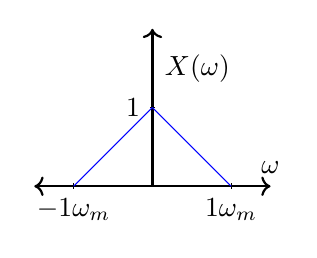
\begin{tikzpicture}
        \draw[thick,<->] (-1.5, 0) -- (1.5,0);
        \draw[thick,->] (0,0) -- (0,2);
        \draw (1.5 cm,1pt) node[anchor=south] {$\omega$};
        \draw (1pt,1.5cm) node[anchor=west] {$X(\omega)$};
        \foreach \x in {-1,1}
            \draw (\x cm,1pt) -- (\x cm,-1pt) node[anchor=north] {$\x\omega_m$};
        \foreach \y in {1}
            \draw (1pt,\y cm) -- (-1pt,\y cm) node[anchor=east] {$\y$};
            \draw[scale=1,domain=0:1,smooth,variable=\x,blue] plot ({\x},{1-\x});
            \draw[scale=1,domain=-1:0,smooth,variable=\x,blue] plot ({\x},{\x+1});
    \end{tikzpicture}  
\end{figure}
There are two major cases: if $\omega_0 > 2\omega_m$ and $\omega_0 < 2\omega_M$.\\
\textbf{Case One: }$\omega_s > 2\omega_m$
\begin{figure}[H]
    \centering
    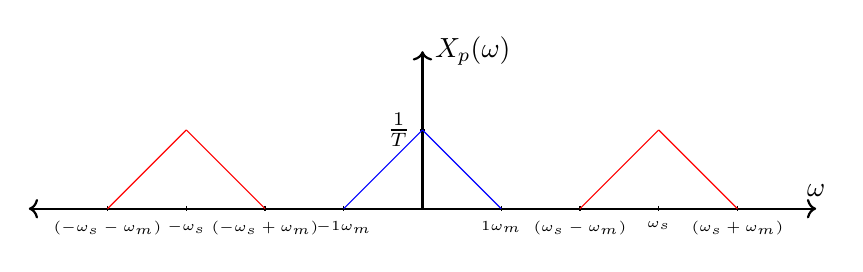
\begin{tikzpicture}
        \draw[thick,<->] (-5, 0) -- (5,0);
        \draw[thick,->] (0,0) -- (0,2);
        \draw (5 cm,1pt) node[anchor=south] {$\omega$};
        \draw (1pt,2cm) node[anchor=west] {$X_p(\omega)$};
        \draw (3 cm,1pt) -- (3 cm,-1pt) node[anchor=north, font=\tiny] {$\omega_s$};
        \draw (-3 cm,1pt) -- (-3 cm,-1pt) node[anchor=north, font=\tiny] {$-\omega_s$};
        \draw (2 cm,1pt) -- (2 cm,-1pt) node[anchor=north, font=\tiny] {$(\omega_s-\omega_m)$};
        \draw (4 cm,1pt) -- (4 cm,-1pt) node[anchor=north, font=\tiny] {$(\omega_s+\omega_m)$};
        \draw (-2 cm,1pt) -- (-2 cm,-1pt) node[anchor=north, font=\tiny] {$(-\omega_s+\omega_m)$};
        \draw (-4 cm,1pt) -- (-4 cm,-1pt) node[anchor=north, font=\tiny] {$(-\omega_s-\omega_m)$};
        \foreach \x in {-1,1}
            \draw (\x cm,1pt) -- (\x cm,-1pt) node[anchor=north, font=\tiny] {$\x\omega_m$};
        \foreach \y in {1}
            \draw (1pt,\y cm) -- (-1pt,\y cm) node[anchor=east] {$\frac{\y}{T}$};
            \draw[scale=1,domain=0:1,smooth,variable=\x,blue] plot ({\x},{1-\x});
            \draw[scale=1,domain=-1:0,smooth,variable=\x,blue] plot ({\x},{\x+1});
            \draw[scale=1,domain=3:4,smooth,variable=\x,red] plot ({\x},{4-\x});
            \draw[scale=1,domain=2:3,smooth,variable=\x,red] plot ({\x},{\x-2});
            \draw[scale=1,domain=-4:-3,smooth,variable=\x,red] plot ({\x},{4+\x});
            \draw[scale=1,domain=-3:-2,smooth,variable=\x,red] plot ({\x},{-2-\x});
    \end{tikzpicture}  
\end{figure}
When $\omega_s > 2\omega_M$, the shifted copies of the original $X(\omega)$ (shown in blue)
do not overlap with each other or which the original copy. If we wanted to recover the original
signal, we could simply apply a low pass filter to isolate the unshifted copy of $X(\omega)$ and
then take the inverse Fourier Transform.\\
\textbf{Case Two: }$\omega_s < 2\omega_m$
\begin{figure}[H]
    \centering
    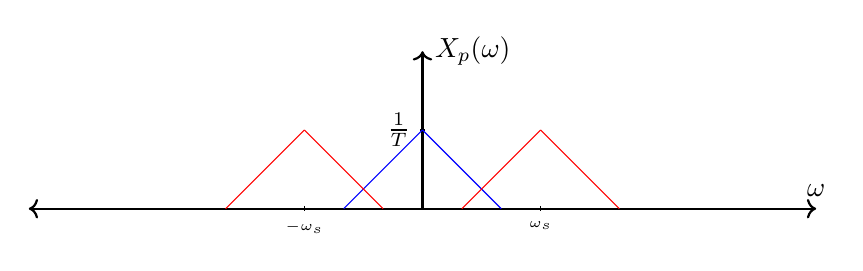
\begin{tikzpicture}
        \draw[thick,<->] (-5, 0) -- (5,0);
        \draw[thick,->] (0,0) -- (0,2);
        \draw (5 cm,1pt) node[anchor=south] {$\omega$};
        \draw (1pt,2cm) node[anchor=west] {$X_p(\omega)$};
        \draw (1.5 cm,1pt) -- (1.5 cm,-1pt) node[anchor=north, font=\tiny] {$\omega_s$};
        \draw (-1.5 cm,1pt) -- (-1.5 cm,-1pt) node[anchor=north, font=\tiny] {$-\omega_s$};
        \foreach \y in {1}
            \draw (1pt,\y cm) -- (-1pt,\y cm) node[anchor=east] {$\frac{\y}{T}$};
            \draw[scale=1,domain=0:1,smooth,variable=\x,blue] plot ({\x},{1-\x});
            \draw[scale=1,domain=-1:0,smooth,variable=\x,blue] plot ({\x},{\x+1});
            \draw[scale=1,domain=1.5:2.5,smooth,variable=\x,red] plot ({\x},{2.5-\x});
            \draw[scale=1,domain=0.5:1.5,smooth,variable=\x,red] plot ({\x},{\x-0.5});
            \draw[scale=1,domain=-2.5:-1.5,smooth,variable=\x,red] plot ({\x},{2.5+\x});
            \draw[scale=1,domain=-1.5:-0.5,smooth,variable=\x,red] plot ({\x},{-0.5-\x});
    \end{tikzpicture}  
\end{figure}
Notice how in this case, the shifted copies overlap with the original $X(\omega)$. This means in our sampled signal, the higher frequency
information is bleeding in with the lower frequency information. This phenomenon is known as aliasing. When aliasing occurs, we cannot simply
apply a low pass filter to isolate the unshifted copy of $X(\omega)$.\\\\
When $\omega_0 = 2\omega_M$, then our ability to reconstruct the original signal depends on the shape of its Fourier Transform. As long as $X_p(k\omega_m)$
are equal to $X(\omega_m)$ and $X(-\omega_m$), then we can apply an LPF because we can isolate the original $X(\omega)$ and take its inverse Fourier Transform.\\\\
Remember that an ideal low pass filter is a square wave in the frequency domain and a sinc in the time domain. Thus if we allow
\[
    X_r(\omega) = X_p(\omega)\cdot \left\{
            \begin{array}{cc}
                T & |\omega| < \frac{\omega_s}{2}\\
                0 & \text{ else }
            \end{array}
        \right\}
\]
then our reconstructed signal will be
$$x_r(t) = x_p(t)*sinc\left(\frac{t}{T}\right) = \sum_{n=-\infty}^{\infty}{X(nT)sinc\left(\frac{t-nT}{T}\right)}$$
This is why we call reconstructing a signal from its samples "sinc interpolation."
This leads us to formulate the Nyquist Theorem.
\begin{theorem}[CT Nyquist Theorem]
    Suppose a continuous signal $x$ is bandlimited and we sample it at a rate of $\omega_s > 2\omega_M$, then the signal $x_r(t)$
    reconstructed by sinc interpolation is exactly $x(t)$
\end{theorem}
\subsection{Discrete Time}
Sampling in discrete time is very much the same as sampling in continuous time. Using a sampling period of $N$
we construct a new signal by taking an impulse train and multiplying elementwise with the original signal.
\begin{align*}
    p[n]=\sum_{n=-\infty}^{\infty}{\delta[n-kN]}\\
    x_p[n] = x[n]p[n] = \sum_{n=-\infty}^{\infty}{x[kN]\delta[n-kN]}\\
    X_p(\omega) = \frac{1}{N}\sum_{k=0}^{N-1}{X(\omega-k\omega_s)}
\end{align*}
Our indices only go from $k$ to $N-1$ in the Fourier Domain because we can only shift a particular number of times
before we start to get repeated copies.
This is the impulse train sampled signal. It has 0's at the unsampled locations. If we want to, we could simply remove those zeros
and get a downsampled signal
$$x_p[n] = x[Nn]$$
Like in continuous time, the reconstructed signal is recovered via sinc interpolation.
$$x_r[n] = \sum_{k=-\infty}^{\infty}{x_p[n]sinc\left(\frac{n-kN}{N}\right)}$$
The Nyquist Theorem in DT will tell us when this works.
\begin{theorem}[DT Nyquist Theorem]
    Suppose a discrete signal $x$ is bandlimited by $\frac{\pi}{N}$ and we sample it at a rate of $\omega_s > 2\omega_M$, then the signal $x_r[n]$
    reconstructed by sinc interpolation is exactly $x[n]$
\end{theorem}
Thus as long as the Nyquist Theorem holds, we can take a downsampled signal and upsample it (i.e reconstruct the missing pieces) by expanding $y$ by a factor
of $N$ and putting $0's$ for padding, and then applying sinc-interpolation to it.
\subsection{Sampling as a System}
Notice that we have two ways of representing our sample signal. We can either write it as a discrete time signal $x_d[n] = x(nT)$
or we can write it as an impulse train $x_p(t)=\sum_{-\infty}^{\infty}{x(nT)\delta(t-nT)}$.
Based on their Fourier Transforms, 
\begin{align*}
    X_d(\Omega)=\sum_{n=-\infty}^{\infty}{x(nT)e^{-j\Omega n}}\\
    X_p(\omega)=\sum_{n=-\infty}^{\infty}{x(nT)e^{-j\omega nT}}
\end{align*}
Thus if we let $\Omega=\omega T$, then we see that these two representations of a signal have the same Fourier Transforms
and thus contain the same information. This means that for some continuous signals, convert them to discrete time via sampling,
use a computer to apply an LTI system, and convert the result back to a CT output. 
\begin{figure}[H]
    \centering
    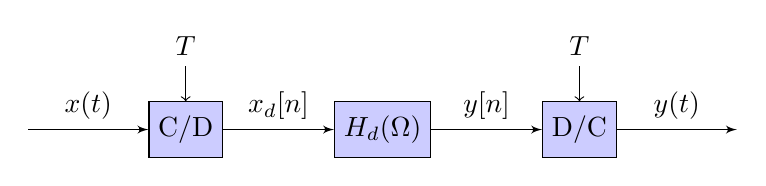
\begin{tikzpicture}[node distance=2.5cm,auto,>=latex']
        \node [int, pin={[init]above:$T$}] (a) {C/D};
        \node (b) [left of=a,node distance=2cm, coordinate] {x(t)};
        \node [int] (c) [right of=a] {$H_d(\Omega)$};
        \node [int, pin={[init]above:$T$}] (d) [right of=c] {D/C};
        \node [coordinate] (end) [right of=d, node distance=2cm]{};
        \path[->] (b) edge node {$x(t)$} (a);
        \path[->] (a) edge node {$x_d[n]$} (c);
        \draw[->] (c) edge node {$y[n]$} (d) ;
        \draw[->] (d) edge node {$y(t)$} (end) ;
    \end{tikzpicture}    
\end{figure}
We must be careful though because
as long as the DT system we apply is LTI, the overall CT system will be linear too, but it will not necessarily be time invariant
because sampling inherently depends on the signal's timing.
\begin{align*}
    Y_d(\Omega) &= H_d(\Omega)X_d(\Omega) = H_d(\Omega)X_p\left(\frac{\Omega}{T}\right)\\
    Y_p(\omega) &= Y_d(\omega T) = H_d(\omega T)X_p(\omega)\\
    Y(\omega) &= \left\{
        \begin{array}{cc}
            T & |\omega| < \frac{\omega_s}{2}\\
            0 & |\omega| \ge \frac{\omega_s}{2}
        \end{array}
        \right\} \cdot Y_p(\omega) = \left\{
            \begin{array}{cc}
                TH_d(\omega T)X_p(\omega) & |\omega| < \frac{\omega_s}{2}\\
                0 & |\omega| \ge \frac{\omega_s}{2}
            \end{array}
            \right\}
\end{align*}
Assuming that the Nyquist theorem holds,
\begin{align*}
    X_p(\omega) &= \frac{1}{T}X(\omega)\\
    \therefore Y(\omega) &= \left\{
        \begin{array}{cc}
            H_d(\omega T)X(\omega) & |\omega| < \frac{\omega_s}{2}\\
            0 & |\omega| \ge \frac{\omega_s}{2}
        \end{array}
    \right\}\\
        \therefore H_{system} &= \left\{\begin{array}{cc}
            H_d(\omega T) & |\omega| < \frac{\omega_s}{2}\\
            0 & |\omega| \ge \frac{\omega_s}{2}
        \end{array}
        \right\}
\end{align*}
This shows us that as long as the Nyquist theorem holds, we can process continuous signals
with a disrete time LTI system and still have the result be LTI.
\section{Appendix}
\subsection{Theory of Distributions}
The Theory of Distributions is the mathematical framework which underlies the generalized Fourier Transforms.
\begin{definition}
    Given a test function $x$, a distribution $T$ operates on $x$ to produce a number $<T,x>$.
\end{definition}
\begin{definition}
    The distrbution induced by a function $g$ is defined as
    $$<T_g, x> = \int_{-\infty}^{\infty}{g(t)^*x(t)dt}$$
\end{definition}
Notice two things:
\begin{itemize}
    \item $<T_g, x>$ is linear
    \item $<\alpha T_g, x> = \alpha^*<T_g, x>$
\end{itemize}
With these definitions, we can now define the Dirac delta in terms of distrubions.
Let $g$ be any function such that
$$\int_{\infty}^{\infty}{g(t)dt} = 1$$
Define $g_\epsilon$ to be
$$g_\epsilon = \frac{1}{\epsilon}g(\frac{t}{\epsilon})$$
Now we can defined $\delta(t) = \lim_{\epsilon \rightarrow 0}{T_{g_\epsilon}}$
$$<\delta, x> = \int_{-\infty}^{\infty}{\delta(t)x(t)dt} = x(0)$$ 
which is the property of the Dirac Delta we want. Now we can define the generalized Fourier Transform
in terms of distributions.
\begin{definition}
    The generalized Continuous Time Fourier Transform of a distrubtion $T$ is
    $$<FT, X> = 2\pi<T, x>$$
    for test function $x$ whose Fourier Transform is $X$
\end{definition}
\end{document}